\documentclass{beamer}
\usetheme{Singapore}
\setbeamertemplate{navigation symbols}{}

\usepackage{graphicx} % Provides the \includegraphics[]{} command

\title{A Comparative Analysis of Constituencies in England and Wales}
\author{Dan Saattrup Nielsen}
\date{\today}

\begin{document}

\begin{frame}[plain]
	\titlepage
\end{frame}

\begin{frame}{What is the problem at hand?}
	\begin{itemize}
		\item Say you have a company in Bristol, and you want to branch out to a different city. Which one do you choose?
    \pause\item You \textit{could} just do like everyone else and head to London. But is that the correct choice? What other options do you have?
    \pause\item There are 650 parliamentary constituencies in the UK. You do not have time to look through every one of them in detail.
	\end{itemize}
\end{frame}

\begin{frame}{What information defines an area?}
  \begin{itemize}
    \item The total population of the area
    \item The average age
    \item The size of the area, to account for population density
    \item House prices in the area, to estimate population wealth
    \item Amount of businesses in the area
    \item The \textit{type} of businesses in the area
    \item The qualifications of the population of the area
    \item Amenities present in the area
  \end{itemize}
\end{frame}

\begin{frame}{Differentiating areas}
  \begin{center}
    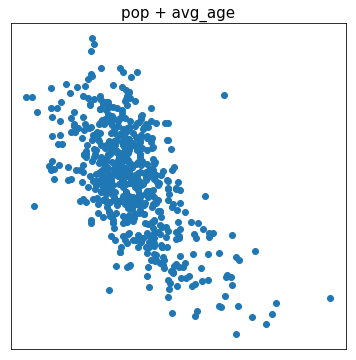
\includegraphics[scale=.40]{../gfx/cluster0.png}
  \end{center}
\end{frame}

\begin{frame}{Differentiating areas}
  \begin{center}
    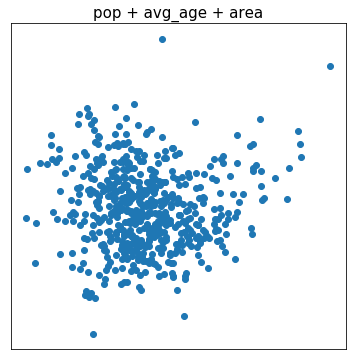
\includegraphics[scale=.40]{../gfx/cluster1.png}
  \end{center}
\end{frame}

\begin{frame}{Differentiating areas}
  \begin{center}
    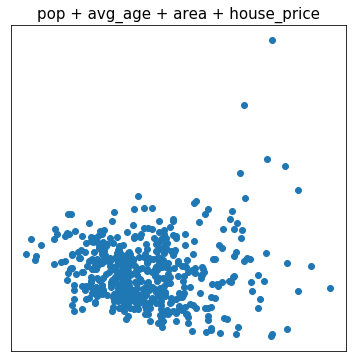
\includegraphics[scale=.40]{../gfx/cluster2.png}
  \end{center}
\end{frame}

\begin{frame}{Differentiating areas}
  \begin{center}
    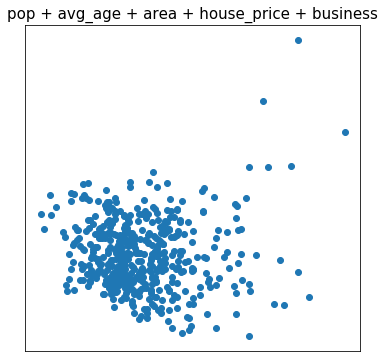
\includegraphics[scale=.40]{../gfx/cluster3.png}
  \end{center}
\end{frame}

\begin{frame}{Differentiating areas}
  \begin{center}
    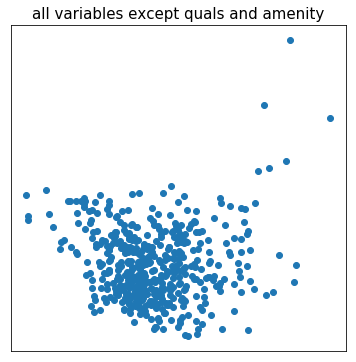
\includegraphics[scale=.40]{../gfx/cluster4.png}
  \end{center}
\end{frame}

\begin{frame}{Differentiating areas}
  \begin{center}
    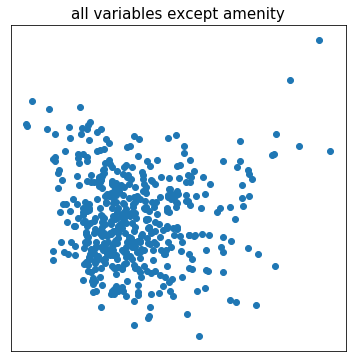
\includegraphics[scale=.40]{../gfx/cluster5.png}
  \end{center}
\end{frame}

\begin{frame}{Differentiating areas}
  \begin{center}
    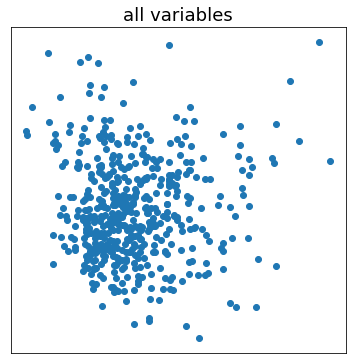
\includegraphics[scale=.40]{../gfx/cluster6.png}
  \end{center}
\end{frame}

\begin{frame}{Applying k-means clustering}
  \begin{center}
    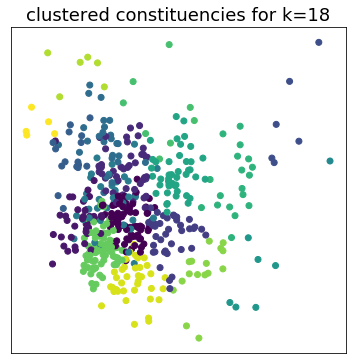
\includegraphics[scale=.40]{../gfx/cluster_colour_small.png}
  \end{center}
\end{frame}

\begin{frame}{Applying k-means clustering}
  \begin{center}
    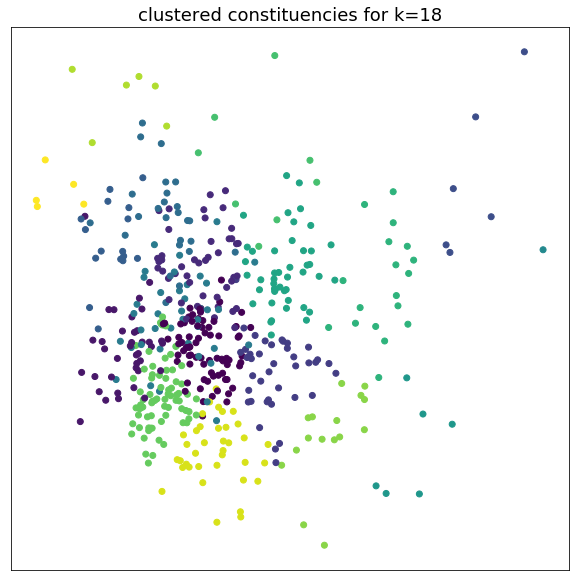
\includegraphics[scale=.35]{../gfx/cluster_colour.png}
  \end{center}
\end{frame}


\begin{frame}{Distribution of clusters}
  \begin{center}
    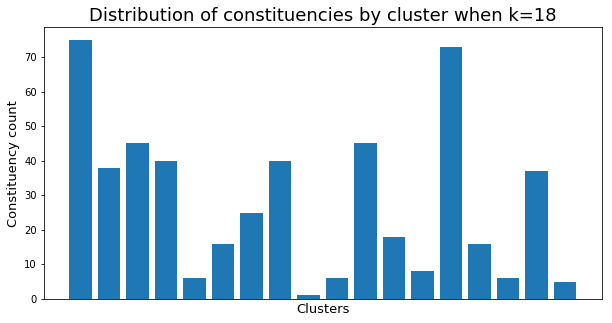
\includegraphics[scale=.50]{../gfx/cluster_dist1.png}
  \end{center}
\end{frame}


\begin{frame}{The resulting similar areas to Bristol}
  \begin{center}
    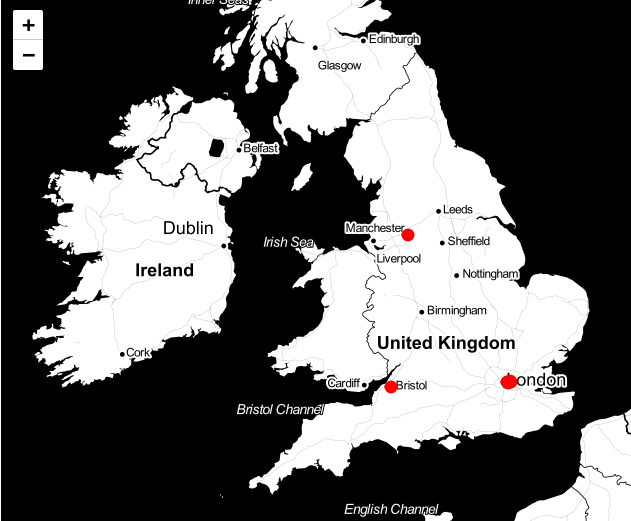
\includegraphics[scale=.43]{../gfx/map0.png}
  \end{center}
\end{frame}

\end{document}
